\section{Об управлении двузвенным манипулятором с приводом} \label{p24}

Рассмотрим манипулятор, моделируемый в виде механической системы, состоящей из неподвижного основания $G_0$ и двух абсолютно жестких звеньев $G_1, G_2$. Элементы конструкции соединены между собой двумя цилиндрическими шарнирами $O_1, O_2$ таким образом, что оба звена могут совершать движения только в горизонтальной плоскости под действием приводов, приложенных в этих шарнирах.

Будем считать, что приводы управляются некоторыми воздействиями $L_{i}$ в соответствии с уравнениями 

\begin{equation} \label{2.14'}
\frac{d M_i}{dt} = L_{i}
\end{equation}

Рассматривается задача построения структуры обратной связи в виде зависимости $L_{i} = L_{i} (t, q, \dot q, M)$ таким образом, чтобы каждое программное движение системы $(q_1 (t), q_2 (t))$ являлось бы асимптотически устойчивым. 

Продемонстрируем решение этой задачи для случая положения равновесия системы

\begin{equation} \label{2.15'}
\dot q_1 = \dot q_2 = 0, \quad q_1 = q_2 = 0, \quad M_1 = M_2 = 0
\end{equation}

Покажем, что такая задача решается управлением приводами со следующим видом обратной связи

\begin{equation}  \label{2.16'}
L_1 = - M_1 - k_1 (\dot q_1 + \beta_1 \sin \frac{q_1}{4}), \quad L_2 = - M_2 - k_2 (\dot q_2 + \beta_2 \sin \frac{q_2}{4})
\end{equation}

где $k_1, k_2, \beta_1, \beta_2 > 0$ есть некоторые постоянные, определяемые из условия стабилизации положения равновесия (\ref{2.15'}).

Для нахождения этих условий применим метод векторых функций Ляпунова [], в соотвтетствии с методикой их построения, представленной в [].

Векторную функцию Ляпунова возьмем в виде
$$
\begin{array}{l}
V_1 = \sqrt{c_1 \sin^2 \frac{q_1}{4} + c_2 \sin^2 \frac{q_2}{4}}, \quad c_1, c_2 > 0\\
V_2 = \sqrt{a_{11} (\dot q_1 + \beta_1 \sin \frac{q_1}{4})^2 + 2 a_{12} (\dot q_1 + \beta_1 \sin \frac{q_1}{4}) (\dot q_2 + \beta_2 \sin \frac{q_2}{4}) + a_{22} (\dot q_2 + \beta_2 \sin \frac{q_2}{4})^2}\\
V_3 = \sqrt{p_{11} (M_1 + k_1 (\dot q_1 + \beta_1 \sin \frac{q_1}{4})^2) + 2 p_{12} (M_1 + k_1 (\dot q_1 + \beta_1 \sin \frac{q_1}{4})) (M_2 + k_2 (\dot q_2 + \beta_2 \sin \frac{q_2}{4})) + p_{22} (M_1 + k_1 (\dot q_2 + \beta_2 \sin \frac{q_2}{4}))^2}\\
a_{11} > 0, a_{11} a_{22} > 0, p_{11} > 0, p_{11} p_{22} - p_{12}^2 > 0
\end{array}
$$ 

Для производной функции $V_1$ в силу (\ref{2.12'}), (\ref{2.13'}), (\ref{2.15'}) 
при $\| q_1 \| \le \Pi, \quad \| q_2 \| \le \Pi$ находим оценку 
$$
\begin{array}{c}
\dot V_1 = \frac{1}{4 V_1} (c_1 \sin \frac{q_1}{4} \cos \frac{q_1}{4} - \dot q_1 + c_2 \sin \frac{q_2}{4} \cos \frac{q_1}{4} \dot q_2) =\\
= \frac{1}{4 V_1} (c_1 \sin \frac{q_1}{4} \cos \frac{q_1}{4} (\dot q_1 + \beta_1 \sin \frac{q_1}{4} - \beta_2 \sin \frac{q_1}{4}) +\\
+ c_2 \sin \frac{q_2}{4} \cos \frac{q_2}{4} (\dot q_2 + \beta_2 \sin \frac{q_2}{4} - \beta_2 \sin \frac{q_2}{4})) \le\\
\le \frac{1}{4 V_1} (\sqrt{c_1 \sin^2 \frac{q_1}{4} + c_2 \sin^2 \frac{q_2}{4}} \sqrt{c_1 (\dot q_1 + \beta_1 \sin \frac{q_1}{4})^2 +\\
+ c_2 (\dot q_2 + \beta_2 \sin \frac{q_2}{4})^2} - \frac{\sqrt{2}}{2} (c_1 \beta_1 \sin^2 \frac{q_1}{4} c_2 \beta_2 \sin^2 \frac{q_2}{4})) \le\\
\le - \alpha_1 V_1 + \alpha_2 V_2, \alpha_1 = \frac{\sqrt{2}}{8} min(\sqrt{c_1} \beta_1, \sqrt{c_2}, \beta_2), \alpha_2 = \frac{1}{4} \sqrt{\lambda_{AC}^{max}}
\end{array}
$$

где $\lambda_{AC}^{max}$ - наибольшее характеристическое значение матрицы $c = diag(c_1, c_2)$ на пучке матриц $A = A(q).$

Для производной от функции $V_2$ в силу (\ref{2.12'}), (\ref{2.13'}), (\ref{2.15'}) имеем более сложную оценку.
$$
\begin{array}{c}
\dot V_2 = \frac{1}{V_2} ((\dot q_1 + \beta_1 \sin \frac{q_1}{4}) ((M_1 + k_1 (\dot q_1 + \beta_1 \sin \frac{q_1}{4})) -\\
- k_1 (\dot q_1 + \beta_1 \sin \frac{q_1}{4}) + \frac{1}{4} a_{11} \beta_2 \cos \frac{q_1}{4} (\dot q_1 + \beta_1 \sin \frac{q_1}{4}) - \frac{1}{4} a_{11} \beta_1^2 \cos \frac{q_1}{4} \sin \frac{q_1}{4}) +\\
+ 2 m_2 l_1 l_2 \sin q_2 (\dot q_2 + \beta_2 \sin \frac{q_2}{4} - \beta_2 \sin \frac{q_2}{4})^2) +\\
+ (\dot q_2 + \beta_2 \sin \frac{q_2}{4}) (M_2 + k_2 (\dot q_2 + \beta_2 \sin \frac{q_2}{4}) -\\
- k_2 (\dot q_2 + \beta_2 \sin \frac{q_1}{4}) + \frac{1}{4} a_{12} \beta_2 \cos \frac{q_2}{4} (\dot q_2 + \beta_2 \sin \frac{q_2}{4}) -\\
- \frac{1}{4} a_{22} \beta_2^2 \cos \frac{q_2}{4} \sin \frac{q_2}{4} -\\
- m_2 l_1 l_2 \sin q_2 (\dot q_1 + \beta_1 \sin \frac{q_1}{4} - \beta_1 \sin \frac{q_1}{4})^2) \le\\
\le \gamma_1 V_1 - \gamma_2 V_2 + \gamma_3 V_3 + \mu_{21} V_1^2 + \mu_{22} V_2^2 + \mu_{23} V_3^2, \gamma_1 =\\
= \frac{p_{max}}{\lambda_{min}}, \gamma_2 = \frac{1}{\lambda_{min}}, \gamma_3 = \frac{1}{4} a_{max} \beta_{max}
\end{array}
$$

где $\mu_{21}, \mu_{22}, \mu_{23}$ зависят от параметров системы и управления.

Для производной функции $V_3$ более сложными вычислениями получим оценку

$\dot V_3 \le V_1 + V_2 - V_3 + \mu_{31} V_1^2 + \mu_{32} V_2^2 + \mu_{33} V_3^2$

$\nu_1 = \frac{2}{\sqrt{\lambda_{min}}} (a_{11} + \| a_{12} \|) \beta_1, \nu_2 = \frac{2}{\sqrt{\lambda_{min}}} (\| a_{12} \| + a_{22}) \beta_1$

$\nu_3 = k - 2 ((a_{11} + \| a_{12} \|) \beta_1 + (\| a_{12} \| + a_{22}) \beta_2), k = \min (k_1, k_2), $

где $\mu_{3i} > 0$ - некоторые коэффициенты, выражаемые через параметры $k_i, \beta_i$.

Стабилизация движения (\ref{2.14'}) согласно теореме об асимптотической устойчивости из [] в самой общей постановке может определяться системой

$\dot y_1 = - \alpha_1 y_1 + \alpha_2 y_2$

$\dot y_2 = \gamma_1 y_1 - \gamma_2 y_2 + \gamma_3 y_3 + \gamma_{31} y_1^2 + \mu_{22} y_2^2 + \mu_{33} y_3^2$

$\dot y_3 = \nu_1 y_1 + \nu_2 y_2 - \nu_3 y_3 + \mu_{31} y_1^2 + \mu_{32} y_2^2 + \mu_{33} y_3^2$

При малых возмущениях стабилизация находится из асимптотической устойчивости линейной системы

$\dot y_1 = - \alpha_1 y_1 + \alpha_2 y_2, \dot y_2 = \gamma_1 y_1 - \gamma_2 y_2 + \gamma_3 y_3, \dot y_3 = \nu_1 y_1 + \nu_2 y_2 - \nu_3 y_3$

Ниже представлены результаты численного моделирования процесса стабилизации положения при следующих численных значениях $\mu_1 = 1, k_1 = 5, \beta_1 = 6, \mu_2 = 1, k_2 = 4, \beta_2 = 7, q_{10} = 0,5, q_2 = 0,8, \dot q_{10} = 0,6, \dot q_{20} = 0,8, M_{10} = 0,9, M_{20} = 0,7, \mu_{20} = 0,7, l_1 = 1 м, l_{g_2} = 0,5 м, I_1 = I_2 = 3,33 кг м 3, m_2 = 10 кг$ 

\begin{figure}[h]
	\centering
	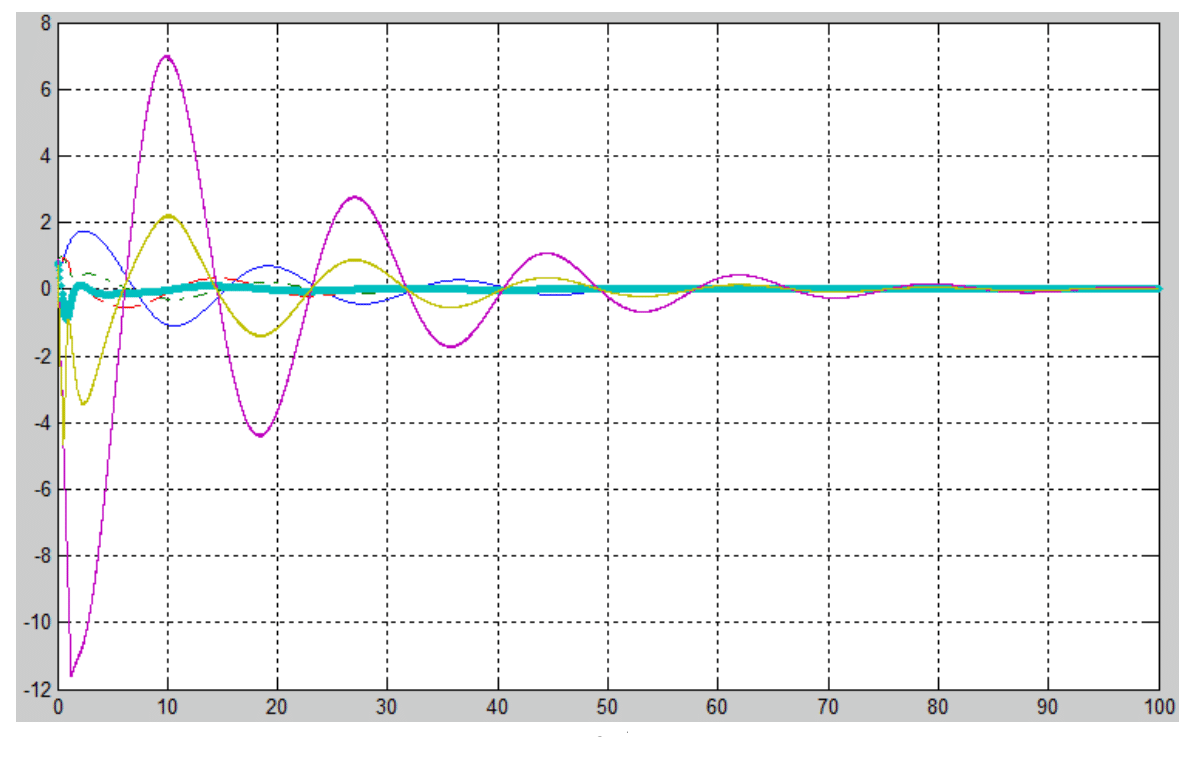
\includegraphics{model3333}
	\caption{Результаты моделирования при управлении (2.16)}
	\label{fig:manip22}
\end{figure}